%----------------------------------------------------------------------------------------
%	PACKAGES AND OTHER DOCUMENT CONFIGURATIONS
%----------------------------------------------------------------------------------------

\documentclass[11pt]{article}
%\input{mydef.tex}
\usepackage{fancyhdr} % Required for custom headers
\usepackage{lastpage} % Required to determine the last page for the footer
\usepackage{extramarks} % Required for headers and footers
\usepackage[usenames,dvipsnames]{color} % Required for custom colors
\usepackage{graphicx} % Required to insert images
\usepackage{listings} % Required for insertion of code
\usepackage{courier} % Required for the courier font
\usepackage{amssymb,amsmath}
\usepackage{amsfonts}
\usepackage{mathtools}
\usepackage{subfigure}
\usepackage{enumitem}
\usepackage{bm}
\usepackage{url}
\usepackage[stable]{footmisc}
\usepackage{booktabs}
\usepackage[square]{natbib}
\usepackage{indentfirst}
%\usepackage[colorlinks, linkcolor=red, anchorcolor=purple, citecolor=blue]{hyperref}
\usepackage{hyperref}

\usepackage{multicol}
\usepackage{multirow}
\usepackage{array}
\newcolumntype{M}[1]{>{\centering\arraybackslash}m{#1}}
\setlength{\columnsep}{1cm}

% Margins
\topmargin=-0.45in
\evensidemargin=0in
\oddsidemargin=0in
\textwidth=6.5in
\textheight=9.0in
\headsep=0.25in
\setlength{\headheight}{13.6pt}
\linespread{1.1} % Line spacing

% Set up the header and footer
\pagestyle{fancy}
\lhead{CS 57800} % Top left header
\chead{Ting Zhang}
\rhead{Howework 1} % Top right header
\lfoot{} % Bottom left footer
\cfoot{} % Bottom center footer
\rfoot{Page\ \thepage\ of\ \protect\pageref{LastPage}} % Bottom right footer
\renewcommand\headrulewidth{0.4pt} % Size of the header rule
\renewcommand\footrulewidth{0.4pt} % Size of the footer rule

\renewcommand*{\thefootnote}{\fnsymbol{footnote}}

\setlength{\parskip}{.2\baselineskip}
%\setlength\parindent{0pt} % Removes all indentation from paragraphs

\title{
\textbf{CS57800 Statistical Machine Learning} \\ \textsc{Homework 1} \\
\normalsize\vspace{0.1in}
}

\author{
	\textbf{Ting Zhang} \\
	School of Industrial Engineering\\
	\texttt{zhan1013@purdue.edu}
}

\date{\today}
%----------------------------------------------------------------------------------------

\begin{document}

\maketitle
%\thispagestyle{empty}

\section{Foundations}
\begin{itemize}
\item[(1)] The normal vectors of the two planes are \(a=(1,1,3)\) and \(b=(1,2,4)\). The vector that is parallel to the intersection line can be computed as:
\begin{equation*}
\begin{split}
l' & =a*b=(1*4-3*2,3*1-1*4,1*2-1*1) \\
 & =(-2,-1,1)
\end{split}
\end{equation*}
Then we need to find a point P, which is on both planes. For example, we can solve the following system with \(x_3=0\) to get a particular P.
%\begin{equation*}
\begin{align*}
& x_1+x_2=4 \\
& x_1+2x_2=5
\end{align*}
%\end{equation*}
So, we get \(x_1=3\) and \(x_2=1\). Therefore, \(P=(3,1,0)\). Then the intersection line can be represented as:
\begin{align*}
&x_1=3-2t \\
&x_2=1-t \\
&x_3=t \\
\end{align*}
\item[(2)] Let's first get the two lines formed by the three points.
\begin{align*}
&\vec{a}=PQ=(1,-1,1)-(0,0,0)=(1,-1,1) \\
&\vec{b}=PR=(4,3,7)-(0,0,0)=(4,3,7)
\end{align*}
Then, the vector orthogonal to the plane of P, Q and R can be computed following:
\begin{equation*}
\begin{split}
\vec{a}\times\vec{b} & =\left| \begin{array}{ccc}
i & j & k \\
1 & -1 & 1 \\
4 & 4 & 7 \end{array} \right| \\
& =\left| \begin{array}{cc}
-1 & 1\\
3 & 7 \end{array} \right|i
-  \left| \begin{array}{cc}
1 & 1\\
4 & 7 \end{array} \right|j
+ \left| \begin{array}{cc}
1 & -1\\
4 & 3 \end{array} \right|k \\
& = -10i-3j+7k
\end{split}
\end{equation*}
Therefore, the vector orthogonal to the plane of P, Q and R is \(\vec{v}=(-10,-3,7)\).
\item[(3)] (a) 
\begin{flalign*}
\frac{df(x)}{dx} & =(x^{\frac{1}{2}})\frac{d(3x^2)}{dx}+(3x^2)(\frac{dx^{\frac{1}{2}}}{dx}) \\
& =x^{\frac{1}{2}}6x+(3x^2)(\frac{1}{2}x^{-\frac{1}{2}}) \\
& =6x^{\frac{3}{2}}+\frac{3}{2}x^{\frac{3}{2}} \\
& =\frac{15}{2}x^{\frac{3}{2}}
\end{flalign*}
(b) 
\begin{equation*}
\begin{split}
\frac{df(x)}{dx} & = \frac{d(e^{2x}+e)^{\frac{1}{2}}}{d(e^{2x}+e)} \frac{d(e^{2x}+e)}{dx} \\
& = \frac{1}{2} (e^{2x}+e)^{-\frac{1}{2}} (2e^{2x})\\
& = e^{2x}(e^{2x}+e)^{-\frac{1}{2}} 
\end{split}
\end{equation*}
(c) 
\begin{equation*}
\begin{split}
\frac{df(x)}{dx} & = \frac{d([\ln (5x^2+9)]^3)}{d(\ln(5x^2+9))} \frac{d(\ln(5x^2+9)}{d(5x^2+9)} \frac{d(5x^2+9)}{dx} \\
& = 3\ln(5x^2+9)^2 \frac{1}{5x^2+9} (10x) \\
& = \frac{30x \ln(5x^2+9)^2}{5x^2+9}
\end{split}
\end{equation*}
\item[(4)] (a)
\begin{equation*}
\frac{\partial f(x,y)}{\partial x} = y^3+2xy^2 
\end{equation*}
\begin{equation*}
\frac{\partial f(x,y)}{\partial y} = 3xy^2+2x^2y
\end{equation*}
(b)
\begin{equation*}
\begin{split}
\frac{\partial f(x,y)}{\partial x} & = \frac{\partial x}{\partial x} e^{2x+3y} + x \frac{\partial (e^{2x+3y})}{\partial x} \\
& = e^{2x+3y} + 2x(e^{2x+3y})\\
& = (2x+1)e^{2x+3y}\\
\end{split}
\end{equation*}
\begin{equation*}
\frac{\partial f(x,y)}{\partial y} = 3xe^{2x+3y}
\end{equation*}
\item[(5)] To compare the grow speed of two function, we can compute the limit of their ratio when n goes to infinity, shown in Eq. (1). If the limit is infinity, then \(f(x)\) grows faster than \(g(x)\); and 0, otherwise.
\begin{equation}
\lim_{x\to\infty} \frac{f(x)}{g(x)}
\end{equation}
Therefore, we perform pairwise comparsions to the functions listed in the question.\\
\begin{itemize}
\item compare \(\log^4\sqrt{n}\) and \(2^{\log_2n}\)\\
\begin{equation*}
 \lim_{n\to\infty} \frac{2^{\log_2n}}{\log^4\sqrt{n}} =  \lim_{n\to\infty} \frac{n}{\frac{1}{16}\log^4n}  =   \lim_{n\to\infty} \frac{16n}{4\log^3n}= \lim_{n\to\infty} \frac{4n}{3\log^2n}= \lim_{n\to\infty} \frac{4n}{6\log^n} = \lim_{n\to\infty} \frac{4n}{6} = +\infty
\end{equation*}
Therefore, \(\log^4\sqrt{n} \prec 2^{\log_2n}\) \\
\item compare \(2^{\log_2n}\) and \(n^{\frac{3}{2}}\log^2n\)
\begin{equation*}
\lim_{n\to\infty} \frac{n^{\frac{3}{2}}\log^2n}{2^{\log_2n}}=\lim_{n\to\infty} \frac{n^{\frac{3}{2}}\log^2n}{n}=\lim_{n\to\infty} n^{\frac{1}{2}}\log^2n=+\infty
\end{equation*}
Therefore, \( 2^{\log_2n}  \prec  n^{\frac{3}{2}}\log^2n    \)\\
\item compare \(n^{\frac{3}{2}}\log^2n\) and \(2^{3\log_2n}\)\\
\begin{equation*}
\lim_{n\to\infty} \frac{2^{3\log_2n}}{n^{\frac{3}{2}}\log^2n}=\lim_{n\to\infty} \frac{n^3}{n^{\frac{3}{2}}\log^2n} = \lim_{n\to\infty} \frac{n^{\frac{3}{2}}}{\log^2n}=\lim_{n\to\infty} \frac{3n^{\frac{3}{2}}}{4\log n} =\lim_{n\to\infty} \frac{9n^{\frac{3}{2}}}{8} =+\infty
\end{equation*}
Therefore, \(n^{\frac{3}{2}}\log^2n \prec 2^{3\log_2n}\)\\
\item compare \(2^{3\log_2n}\) and \(2^n\)\\
\begin{equation*}
\lim_{n\to\infty} \frac{2^{3\log_2n}}{2^n}=\lim_{n\to\infty} \frac{n^3}{2^n} = \lim_{n\to\infty} \frac{3n^2}{2^n\log2}= \lim_{n\to\infty} \frac{6}{2^n\log^32}=0
\end{equation*}
Therefore,  \(2^{3\log_2n} \prec 2^n \)\\
\item compare \(2^n\) and \(\frac{5}{3}^{2n}\)\\
\begin{equation*}
\lim_{n\to\infty} \frac{\frac{5}{3}^{2n}}{2^n} = \lim_{n\to\infty} \frac{(\frac{25}{9})^n}{2^n} = \lim_{n\to\infty} (\frac{25}{18})^n = +\infty
\end{equation*}
Therefore, we have \(2^n \prec \frac{5}{3}^{2n} \)\\
\end{itemize}
Since \(10^8\) does not grow, we can have a sequence shown below:\\
\( 10^8 \prec \log^4\sqrt{n} \prec 2^{\log_2n} \prec  n^{\frac{3}{2}}\log^2n  \prec  2^{3\log_2n} \prec 2^n \prec \frac{5}{3}^{2n} \)
\item[(6)] (a) Define the three rolls as \(X_1\), \(X_2\) and \(X_3\). We can compute the expected value for each roll as
\begin{equation*}
E(X_i)=\frac{1}{6} \sum_{j=1}^{6} j = \frac{7}{2} \quad \textrm{for} \quad i=1,2,3
\end{equation*}
Therefore, the expected value of the sum of the rolls would be 
\begin{equation*}
E(\sum_{i=1}^{3} X_i)=\frac{21}{2}
\end{equation*}
(b) To compute the expected value of the product of the rolls, we can simply multiply their individual expected value since these rolls are independent.
\begin{equation*}
E(X_1X_2X_3)=E(X_1)E(X_2)E(X_3)=(\frac{7}{2})^3=\frac{343}{8}
\end{equation*}
(c) The variance of one roll can be computed as 
\begin{equation*}
V(X_i)=E(X_i^2)-E(X_i)^2 = \frac{1}{6}\sum_{j=1}^{6} j^2 - (\frac{7}{2})^2 = \frac{35}{12}
\end{equation*}
Therefore, the variance of the sum of rolls is
\begin{equation*}
V(\sum_{i=1}^{3} X_i)=\frac{35}{4}
\end{equation*}
\end{itemize}

\section{Programming Report}
In this task, a decision tree was implemented to classify the type of growth of breast cancer. A basic decision tree algorithm \(ID_3\) was implemented, with two different strategies dealing with overfitting. The two strategies including: (1) statically fix the depth of the tree, and (2) post prune the tree after the full tree is established following algorithm \(ID_3\).

\subsection{Decision Tree Construction}
To build a decision tree classifier, we need to first train a decision tree based on training dataset, tune hyper-parameters using validation set, and at last, build a classifier using the constructed decision tree. In the training algorithm, information gain was computed to select the most salient attribute. To compute the informaiton gain, a subset of the original training dataset was extracted based on attributes and their values. The scheme of majority votes was applied when the last available attribute can't determine the type explicitly. While constructing the decision tree, the label of majority votes for every node is computed and applied later in the classification algorithm when there is no available label.\\
To avoid overfitting, two strategies were applied:
\begin{itemize}
\item[(1)] Fixed depth of decision tree\\
Shorter trees are more preferred than deep trees, since they may be more generalizable. Therefore, the depth of trees were limited in this approach. While training a decision tree, the  algorithm stops and build leaves when it reached the maximum depth. Majority votes were used to decide the label. The depth of a decision tree is then becoming a hyper-parameter and can be tuned using a validation set (see explanations in next section).
\item[(2)] Post Pruning\\
The other approach applied to avoid overfitting is post pruning. A full tree was first built using the basic decision tree algorithm. A pruning algorithm was then applied for each non-leaf node from the bottom of a tree to the root. Each non-leaf node was substituted with the label of the majority votes. The prunine process stoped when the accuracy of validation set decreases.
\end{itemize}

\subsection{Experiments and Results}
Experiments were conducted following three scenarios: (1) the basic decision tree, (2) decision tree with fixed depth, and (3) decision tree with post pruning. The results of each experiment are presented below. Table \ref{table:sum} summarizes the results of three strategies, including the depth of the tree, and the accuracy of training, validating and testing dataset. %Table 2 presents the incorrectly classified tuples in each dataset for every strategy.
\begin{table}[htdp]
\centering
\caption{Summary of depth and accuracies of different approaches.}
\label{table:sum}
\begin{tabular}{lllll}
\hline
\multirow{2}{*}{} & \multicolumn{1}{c}{\multirow{2}{*}{Depth}} & \multicolumn{3}{l}{Accuracy}    \\ 
                  & \multicolumn{1}{c}{}                       & Training & Validation & Testing \\ \hline 
\(ID_3\)               & 8                                          & 0.983    & 0.85       & 0.95    \\
Fixed Depth       & 3                                          & 0.933    & 0.85       & 0.95    \\
Pruning           & 3                                          &    0.917     & 0.85       & 0.95 \\ \hline
\end{tabular}
\end{table}
\begin{itemize}
\item[(1)] Basic decision tree\\
Following the \(ID_3\) algorithm, the resultant decision tree is of depth 8. The accuracy of training, validating and testing dataset are: 0.983, 0.80 and 0.95. 
\item[(2)] Decision tree with fixed depth\\
In this experiment, hyper-parameter \(depth\) was tuned from 8 to 1. The corresponding accuracies of training and validating dataset are shown in Figure~\ref{fig:depth}. To avoid overfitting, while the accuracy of validation set and training set keep climbing, a depth of 2 or 3 can be a good choice. In this case, \(depth=3\) is selected. The accuracy of testing set with the decision tree of depth 3 is 0.95, which remains the same as the above basic decision tree of depth 8. 

Looking into the specific tree structures, it can be observed that the attribute "Uniformity of Cell Size" plays an important role in deciding the type of growth of breast cancer. When \(depth=2\), only this attribute was applied to determine the type of growth of breast cancer. And it reached accuracy of 0.883 and 0.80 for training and validation dataset. Besides this attribute, there are four other attributes which can be considered as key factors, including "Clump Thickness", "Uniformity of Cell Shape", "Marginal Adhesion" and "Bare Nuclei". 
\item[(3)] Decision tree with post pruning\\
In this section, a pruned decision tree was constructed. After pruning to \(depth=2\), the accuracy of validation set decreased from 0.85 to 0.80, therefore, the pruned tree with \(depth=3\) is selected, and the accuracy of testing test is 0.95, which also remains the same as the basic decision tree of depth 8.
\end{itemize}

\begin{figure}[h]
    \centering
    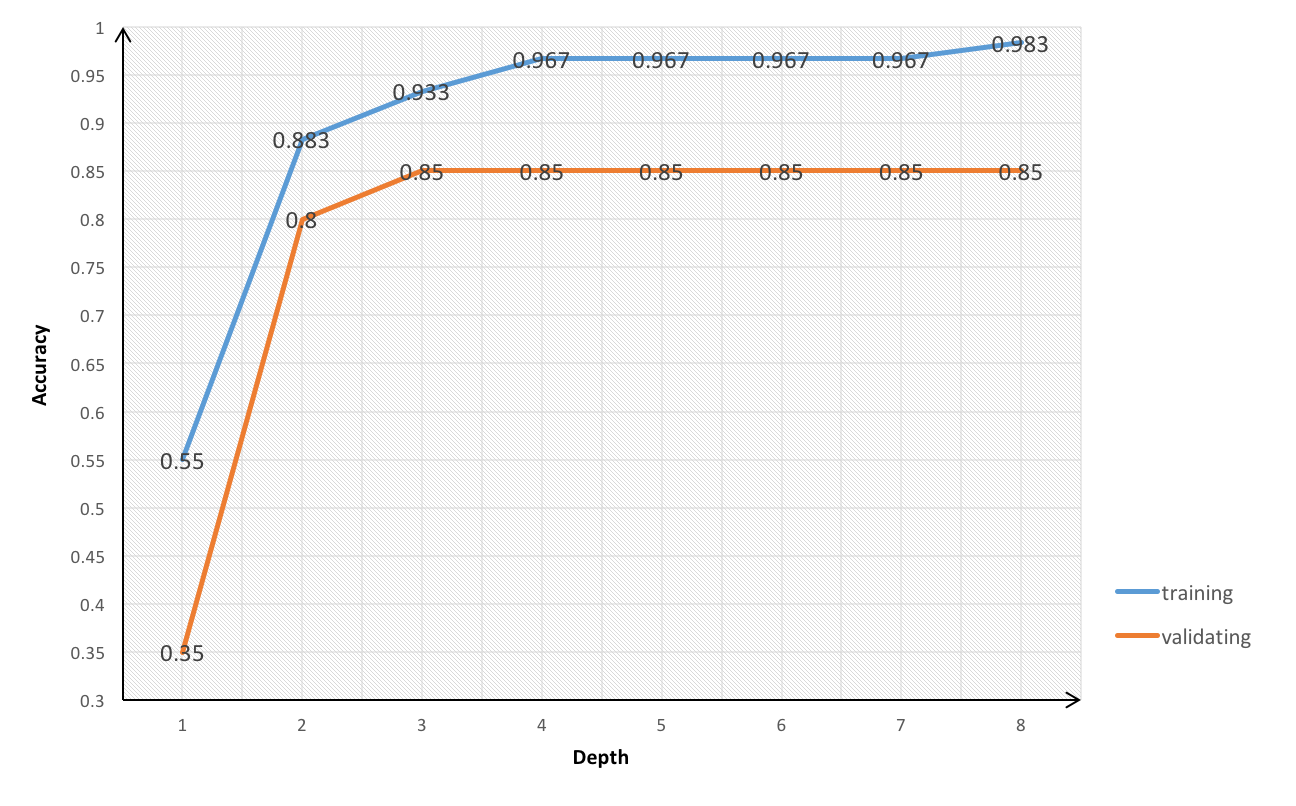
\includegraphics[width=0.8\textwidth]{depth.png}
    \caption{Accuracy of training and validation set with depth from 1 to 8}
    \label{fig:depth}
\end{figure}


\subsubsection{Comparison between strategies}
Comparing these three strategies to build a decision tree, setting a fixed depth and post pruning indicate some level of effectiveness and efficiency, while keepping a relatively shorter tree. Whiling comparing the two strategies to avoid overfitting, it is hard to say which one works better. And the decision tree constructed following these two strategies were the same, in this case. To compare these two strategies, larger dataset may be needed.

\subsection{Discussion}
In this task, a basic decision tree based on \(ID_3\) algorithm was implemented, and two approaches to avoid overfitting were also investigated. Besides the observations found above, it can be seen from the structures of the decision trees generated by all three methods, suffered from having too many leaves with the same label, while the predicted label can only be boolean. A future work to combine the leaves and refine these trees with less nodes may be a contribution to improve the efficiency of the algorithm.

%\nocite{*}
%\bibliographystyle{plainnat}
%\bibliography{all}

\end{document}
